% Options for packages loaded elsewhere
\PassOptionsToPackage{unicode}{hyperref}
\PassOptionsToPackage{hyphens}{url}
\PassOptionsToPackage{dvipsnames,svgnames,x11names}{xcolor}
%
\documentclass[
]{article}
\usepackage{amsmath,amssymb}
\usepackage{iftex}
\ifPDFTeX
  \usepackage[T1]{fontenc}
  \usepackage[utf8]{inputenc}
  \usepackage{textcomp} % provide euro and other symbols
\else % if luatex or xetex
  \usepackage{unicode-math} % this also loads fontspec
  \defaultfontfeatures{Scale=MatchLowercase}
  \defaultfontfeatures[\rmfamily]{Ligatures=TeX,Scale=1}
\fi
\usepackage{lmodern}
\ifPDFTeX\else
  % xetex/luatex font selection
\fi
% Use upquote if available, for straight quotes in verbatim environments
\IfFileExists{upquote.sty}{\usepackage{upquote}}{}
\IfFileExists{microtype.sty}{% use microtype if available
  \usepackage[]{microtype}
  \UseMicrotypeSet[protrusion]{basicmath} % disable protrusion for tt fonts
}{}
\makeatletter
\@ifundefined{KOMAClassName}{% if non-KOMA class
  \IfFileExists{parskip.sty}{%
    \usepackage{parskip}
  }{% else
    \setlength{\parindent}{0pt}
    \setlength{\parskip}{6pt plus 2pt minus 1pt}}
}{% if KOMA class
  \KOMAoptions{parskip=half}}
\makeatother
\usepackage{xcolor}
\usepackage[margin=1in]{geometry}
\usepackage{graphicx}
\makeatletter
\def\maxwidth{\ifdim\Gin@nat@width>\linewidth\linewidth\else\Gin@nat@width\fi}
\def\maxheight{\ifdim\Gin@nat@height>\textheight\textheight\else\Gin@nat@height\fi}
\makeatother
% Scale images if necessary, so that they will not overflow the page
% margins by default, and it is still possible to overwrite the defaults
% using explicit options in \includegraphics[width, height, ...]{}
\setkeys{Gin}{width=\maxwidth,height=\maxheight,keepaspectratio}
% Set default figure placement to htbp
\makeatletter
\def\fps@figure{htbp}
\makeatother
\setlength{\emergencystretch}{3em} % prevent overfull lines
\providecommand{\tightlist}{%
  \setlength{\itemsep}{0pt}\setlength{\parskip}{0pt}}
\setcounter{secnumdepth}{5}
% definitions for citeproc citations
\NewDocumentCommand\citeproctext{}{}
\NewDocumentCommand\citeproc{mm}{%
  \begingroup\def\citeproctext{#2}\cite{#1}\endgroup}
\makeatletter
 % allow citations to break across lines
 \let\@cite@ofmt\@firstofone
 % avoid brackets around text for \cite:
 \def\@biblabel#1{}
 \def\@cite#1#2{{#1\if@tempswa , #2\fi}}
\makeatother
\newlength{\cslhangindent}
\setlength{\cslhangindent}{1.5em}
\newlength{\csllabelwidth}
\setlength{\csllabelwidth}{3em}
\newenvironment{CSLReferences}[2] % #1 hanging-indent, #2 entry-spacing
 {\begin{list}{}{%
  \setlength{\itemindent}{0pt}
  \setlength{\leftmargin}{0pt}
  \setlength{\parsep}{0pt}
  % turn on hanging indent if param 1 is 1
  \ifodd #1
   \setlength{\leftmargin}{\cslhangindent}
   \setlength{\itemindent}{-1\cslhangindent}
  \fi
  % set entry spacing
  \setlength{\itemsep}{#2\baselineskip}}}
 {\end{list}}
\usepackage{calc}
\newcommand{\CSLBlock}[1]{\hfill\break\parbox[t]{\linewidth}{\strut\ignorespaces#1\strut}}
\newcommand{\CSLLeftMargin}[1]{\parbox[t]{\csllabelwidth}{\strut#1\strut}}
\newcommand{\CSLRightInline}[1]{\parbox[t]{\linewidth - \csllabelwidth}{\strut#1\strut}}
\newcommand{\CSLIndent}[1]{\hspace{\cslhangindent}#1}
\ifLuaTeX
\usepackage[bidi=basic]{babel}
\else
\usepackage[bidi=default]{babel}
\fi
\babelprovide[main,import]{french}
% get rid of language-specific shorthands (see #6817):
\let\LanguageShortHands\languageshorthands
\def\languageshorthands#1{}
\usepackage{amsmath} \usepackage{geometry} \usepackage{pdfpages} \usepackage{fontspec} \usepackage{pdfpages} \usepackage{graphicx} \usepackage{amsmath} \usepackage{atbegshi} \usepackage{fancyhdr} \usepackage{tocloft} \usepackage{tcolorbox} \usepackage{xcolor} \definecolor{bleu}{RGB}{0,0,255} \usepackage{everypage} \usepackage{everypage} \usepackage{graphicx} \usepackage{fancyhdr} \pagestyle{fancy} \definecolor{mybrown}{RGB}{139,69,19} \fancyhead[R]{}
\usepackage{booktabs}
\usepackage{longtable}
\usepackage{array}
\usepackage{multirow}
\usepackage{wrapfig}
\usepackage{float}
\usepackage{colortbl}
\usepackage{pdflscape}
\usepackage{tabu}
\usepackage{threeparttable}
\usepackage{threeparttablex}
\usepackage[normalem]{ulem}
\usepackage{makecell}
\usepackage{xcolor}
\ifLuaTeX
  \usepackage{selnolig}  % disable illegal ligatures
\fi
\usepackage{bookmark}
\IfFileExists{xurl.sty}{\usepackage{xurl}}{} % add URL line breaks if available
\urlstyle{same}
\hypersetup{
  pdflang={fr},
  colorlinks=true,
  linkcolor={Maroon},
  filecolor={Maroon},
  citecolor={Blue},
  urlcolor={blue},
  pdfcreator={LaTeX via pandoc}}

\author{}
\date{\vspace{-2.5em}}

\begin{document}

\setcounter{tocdepth}{5}                
\renewcommand\contentsname{\begin{center}\textcolor{brown}{Sommaire}\end{center}}
\AtBeginShipout{
  \ifnum\value{page}=1\thispagestyle{empty}\fi}
\pagestyle{fancy}
\fancyhf{}
\renewcommand{\headrulewidth}{0.4pt}
\renewcommand{\footrulewidth}{0.4pt}
\fancyhead[L]{Elèves Ingénieurs}
\fancyhead[R]{\textcolor{brown}{@Alex, Ali, Richard \& Toussaint}}
\fancyfoot[C]{\thepage}
\fancyfoot[L]{Mars 2025}
\fancyfoot[R]{Projet Statistique}
\AddEverypageHook{
  \ifnum\value{page}>1 
    \fancyhead[L]{Elèves Ingénieurs}
    \fancyhead[R]{\textcolor{brown}{@Alex, Ali, Richard \& Toussaint}}
    \fancyfoot[C]{\thepage}
    \fancyfoot[L]{Mars 2025}
    \fancyfoot[R]{Projet Statistique}
  \else
    \fancyhead[L]{} 
    \fancyhead[R]{}
    \fancyfoot[C]{}
    \fancyfoot[R]{}
  \fi
}

\tableofcontents

\newpage

\renewcommand\listtablename{\begin{center}\textcolor{brown}{Liste des Tableaux}\end{center}}
\renewcommand\listfigurename{\begin{center}\textcolor{brown}{Liste des Figures}\end{center}}

\setlength{\cftfignumwidth}{3em}
\setlength{\cfttabnumwidth}{3em}

\listoftables

\newpage

\listoffigures

\newpage

\section{Introduction}\label{introduction}

La répartition géographique des besoins en soins de santé est un enjeu
majeur pour les politiques publiques, notamment en ce qui concerne
l'accès aux services de médecine de ville. Les inégalités territoriales
dans l'offre et la demande de soins peuvent entraîner des disparités
significatives en matière de santé, affectant particulièrement les
populations vivant dans des zones sous-dotées en professionnels de
santé. Comprendre ces dynamiques spatiales et socio-démographiques est
essentiel pour identifier les zones prioritaires et orienter les
décisions en matière d'allocation des ressources.

Dans ce contexte, ce travail propose une modélisation du nombre de
consultations en médecine de ville à l'échelle communale, en tenant
compte des caractéristiques démographiques, socio-économiques et
spatiales des communes. L'objectif est double : d'une part, analyser les
facteurs influençant la demande de soins, et d'autre part, identifier
les zones susceptibles de dépasser un seuil critique de ``désert
médical''. Pour ce faire, nous nous appuierons sur une base de données
riche et variée, comprenant des informations issues du Système National
des Données de Santé (SNDS) pour la période 2018-2022, ainsi que des
indicateurs socio-démographiques et géographiques.

Notre approche méthodologique repose sur une combinaison de techniques
statistiques et spatiales. Nous commencerons par une analyse descriptive
et cartographique des données pour visualiser les tendances et les
disparités territoriales. Ensuite, nous utiliserons des modèles de
régression de Poisson pour modéliser le nombre de consultations
annuelles, en tenant compte des effets fixes (caractéristiques des
communes) et des effets aléatoires (variations spatiales). Enfin, une
régression logistique binaire sera employée pour évaluer la probabilité
qu'une commune dépasse un seuil prédéfini de ``désert médical''.

Ce travail s'inscrit dans une perspective à la fois académique et
opérationnelle. Sur le plan académique, il contribue à l'étude des
inégalités territoriales en santé en proposant une méthodologie robuste
pour l'analyse spatiale des données de soins. Sur le plan opérationnel,
il fournit des outils pour identifier les zones prioritaires et soutenir
la prise de décision en matière de politiques de santé publique.

\section{Présentation du contexte}\label{pruxe9sentation-du-contexte}

\subsection{Intérêt de l'étude}\label{intuxe9ruxeat-de-luxe9tude}

\subsection{Cadre conceptuel de
l'étude}\label{cadre-conceptuel-de-luxe9tude}

Dans cette partie, nous allons définir certainses notions clés qui
apparaissent dans notre étude entre autres, le nombre de visites, le
nombre de visites espérés ainsi que le taux de visite.

\begin{enumerate}
\def\labelenumi{\arabic{enumi}.}
\tightlist
\item
  Nombre de visites espérés
\end{enumerate}

Le nombre de visite espérés, terme qui apparaitra dans notre
modélisation est le nombre de visite qu'il y aurait eu dans chaque
commune si le taux de visite était le même dans dans ces dernières. En
d'autres terme si \(r\) est le taux moyen de visite alors, le nombre de
visite escompté noté \(\mu\) est calculé par :

\[ \mu_i = r * P_i\]

où \(P_i\) est le nombre d'habitants dans la commune \(i\)

\begin{enumerate}
\def\labelenumi{\arabic{enumi}.}
\setcounter{enumi}{1}
\tightlist
\item
  Taux de visite
\end{enumerate}

Le taux de visite n'est rien d'autre que le nombre moyen de visite dans
chaque commune. IL est calculé en divisant le nombre de visite par la
population de la commune en question. En d'autres termes, il s'agit du
nombre de visites que chaque habitant de la commune a effectué en
moyenne.

\[\tau_i = \frac{n_i}{P_i}\]

où \(\tau_i\) et \(n_i\) sont respectivement le taux et le nombre de
visite de la commune \(i\).

\subsection{Revue de littérature}\label{revue-de-littuxe9rature}

La modélisation des visites dans les hôpitaux est cruciale pour
comprendre les dynamiques de la santé publique et pour optimiser la
gestion des ressources médicales. Dans ce contexte, les modèles de
régression de type Poisson généraux, en particulier les modèles mixtes
généralisés (GLMM), sont souvent utilisés pour gérer les données de
comptage, en tenant compte des spécificités démographiques et
géographiques des agglomérations, ici définies par les communes.

Les recherches antérieures, comme celles de Mohebbi et al.~(2011),
montrent l'importance d'intégrer des effets spatiaux dans les modèles de
comptage, surtout lorsqu'on évalue des phénomènes tels que le cancer
œsophagien (EC) dans des provinces spécifiques. Leur étude souligne
comment la non-prise en compte de l'autocorrélation spatiale peut
conduire à une estimation biaisée des effets des variables
socio-économiques sur l'incidence des maladies. Ce phénomène pourrait
également s'appliquer à la modélisation des visites à l'hôpital, où
certains facteurs ouent un rôle significatif.

Selon l'article, trois structures d'autocorrélation peuvent être
appliquées dans le cadre de la régression Poisson lorsqu'on traite des
données de comptage. Ces modèles comprennent :

\begin{enumerate}
\def\labelenumi{\arabic{enumi}.}
\item
  \textbf{Modèle Poisson avec effets aléatoires non spatiaux} : Bien
  qu'utiles, ces modèles négligent l'autocorrélation spatiale, ce qui
  peut conduire à une sous-estimation des erreurs standard.
\item
  \textbf{Modèle avec effets aléatoires spatiaux basés sur la distance}
  : Ce modèle prend en compte l'influence des agglomérations voisines,
  mais peut ne pas capturer efficacement l'hétérogénéité locale.
\item
  \textbf{Modèle avec effets aléatoires de type voisinage} : Utilisant
  la structure conditionnelle autorégressive (CAR), ce modèle est le
  plus adapté pour les données spatiales en intégrant les interactions
  entre les communes. Pour notre étude, le modèle avec effets aléatoires
  de type voisinage est recommandé pour la modélisation du nombre de
  visites à l'hôpital en France, car il permet de mieux prendre en
  compte l'effet de proximité entre communes.
\end{enumerate}

L'application des principes issus de l'article de Mohebbi et al.~peut
enrichir notre étude sur la fréquentation des hôpitaux en France. En
intégrant des effets aléatoires spatiaux adaptés à la structure des
données, nous pouvons réaliser des estimations plus précises et utiles
pour la planification hospitalière.

En ce qui concerne les facteurs explicatifs du nombre de visite dans les
hopitaux, plusieurs études se sont penchées sur ce sujet. De nombreuses
études ont montré que le nombre de consultations médicales est influencé
par divers facteurs sociodémographiques, allant des caractéristiques
individuelles aux contextes socio-économiques et territoriaux.

\begin{enumerate}
\def\labelenumi{\arabic{enumi}.}
\tightlist
\item
  Influence de l'âge et du sexe
\end{enumerate}

L'âge constitue un déterminant majeur du recours aux soins. Les
personnes âgées, en particulier celles de 65 à 79 ans, consultent plus
fréquemment en raison de la prévalence accrue de maladies chroniques et
du suivi médical nécessaire à leur prise en charge (Canada 2022). En
revanche, la population jeune et en bonne santé présente une utilisation
plus sporadique des services médicaux. Le sexe est également un facteur
différenciant important. De manière générale, les femmes consultent plus
fréquemment que les hommes. Cette différence est attribuée aux besoins
spécifiques en santé reproductive, mais aussi à une plus grande
propension à rechercher des soins préventifs (publique 2024). En
revanche, les hommes, notamment dans les catégories
socio-professionnelles les plus actives, ont tendance à sous-utiliser
les services de soins, ce qui peut entraîner des diagnostics plus
tardifs et des complications médicales accrues.

\begin{enumerate}
\def\labelenumi{\arabic{enumi}.}
\setcounter{enumi}{1}
\tightlist
\item
  Impact du statut socio-économique et du niveau d'éducation
\end{enumerate}

Le revenu et la précarité économique influencent considérablement
l'accès aux soins. Les individus à revenu élevé bénéficient généralement
d'un meilleur accès aux consultations médicales, notamment grâce à une
plus grande couverture sociale et des assurances complémentaires leur
permettant de réduire les coûts associés aux soins (Santé 2023). À
l'inverse, les personnes en situation de précarité rencontrent des
obstacles financiers, administratifs et culturels qui limitent leur
recours aux soins, malgré des besoins souvent accrus en raison de
conditions de vie plus précaires. Le niveau d'éducation joue un rôle clé
dans la fréquentation des services de santé. Une instruction plus élevée
est associée à une meilleure connaissance des risques sanitaires et à
une adoption plus proactive des comportements de prévention, ce qui
entraîne un recours plus fréquent aux soins médicaux (Santé 2023). En
revanche, un faible niveau d'éducation est souvent corrélé à un moindre
suivi médical et à une utilisation plus tardive des services de soins,
notamment en cas de complications.

\begin{enumerate}
\def\labelenumi{\arabic{enumi}.}
\setcounter{enumi}{2}
\tightlist
\item
  Influence du contexte familial et de l'environnement social
\end{enumerate}

L'état matrimonial influence également la fréquence des consultations
médicales. Les personnes mariées ou vivant en couple consultent
davantage, bénéficiant du soutien d'un conjoint qui peut inciter à
prendre soin de sa santé et à consulter régulièrement un médecin (Canada
2022). Par ailleurs, l'accès à un médecin traitant ou de famille
constitue un déterminant important. Les patients disposant d'un suivi
médical régulier sont plus enclins à effectuer des consultations
préventives et à être orientés rapidement vers des spécialistes si
nécessaire (Canada 2022).

\begin{enumerate}
\def\labelenumi{\arabic{enumi}.}
\setcounter{enumi}{3}
\tightlist
\item
  Perception de l'état de santé et accès géographique aux soins
\end{enumerate}

La perception de la santé est un facteur déterminant du recours aux
soins. Les individus qui considèrent leur état de santé comme excellent
ou très bon consultent rarement, tandis que ceux qui ont une perception
négative de leur état de santé ont tendance à multiplier les visites
médicales (Canada 2022). Enfin, les inégalités spatiales dans l'accès
aux soins modulent également la fréquence des consultations. En milieu
urbain, la densité médicale plus élevée facilite l'accès aux services de
soins, tandis qu'en zones rurales ou médicalement sous-dotées, les
délais d'attente et les distances à parcourir constituent des freins
majeurs (Irdes 2020).

\section{Méthodologie}\label{muxe9thodologie}

Dans le cadre de cette étude, nous cherchons à modéliser le nombre de
consultations médicales en prenant en compte les caractéristiques
socio-économiques et spatiales des communes. La littérature suggère que
les modèles de régression de Poisson et ses variantes avec effets
aléatoires sont particulièrement adaptés aux données de comptage, tout
en tenant compte de l'hétérogénéité locale et des dépendances spatiales.
Ainsi, nous proposons une approche combinant les modèles de régression
de Poisson standard et les modèles mixtes généralisés pour mieux
comprendre les dynamiques d'accès aux soins.

\subsection{Modélisation du nombre de visites de médécins
généralistes}\label{moduxe9lisation-du-nombre-de-visites-de-muxe9duxe9cins-guxe9nuxe9ralistes}

\subsubsection{Modèle de régression de
Poisson}\label{moduxe8le-de-ruxe9gression-de-poisson}

La régression de Poisson est un type de modèle linéaire généralisé (GLM)
utilisé pour modéliser des données de comptage. La distribution de
Poisson suppose que la variance est égale à la moyenne, ce qui est
souvent approprié pour des données de comptage. Le modèle de base est :

\[
\log(\mu_i) = \beta_0 + \beta_1 X_{i1} + \beta_2 X_{i2} + \dots + \beta_p X_{ip} = (X\beta)_i
\]

où \(\mu_i\) est le nombre attendu de cas pour l'observation \(i\),
\(X_{ij}\) sont les variables explicatives, et \(\beta_j\) sont les
coefficients à estimer. Toutefois, ce modèle suppose une indépendance
entre observations, ce qui peut ne pas être réaliste en présence de
corrélation spatiale ou d'hétérogénéité non observée.

\subsubsection{Modèles de Régression de Poisson avec effets
aléatoires}\label{moduxe8les-de-ruxe9gression-de-poisson-avec-effets-aluxe9atoires}

Afin de mieux capter l'hétérogénéité entre les communes, nous
introduisons des modèles avec effets aléatoires. Ces modèles permettent
de prendre en compte des facteurs non observés qui influencent le nombre
de consultations.

Un effet aléatoire \(v_i\) capture l'effet d'hétérogénéité non mesurable
qui influence les résultats dans chaque agglomération. Il peut être
considéré comme une variation spécifique à l'agglomération qui n'est pas
expliquée par les covariables observées dans le modèle (comme les
facteurs socio-économiques).

\paragraph{Régression de Poisson avec effets aléatoires non
spatiaux}\label{ruxe9gression-de-poisson-avec-effets-aluxe9atoires-non-spatiaux}

La formulation générale de ce modèle peut être écrite comme suit :

\[
\log(\mu_i) = \log(E_i) + (X\beta)_i + u_i
\]

où :

\begin{itemize}
\tightlist
\item
  \(\mu_i\) est la moyenne du nombre de visites pour l'agglomération
  \(i\),
\item
  \(E_i\) est la taille de la population de l'agglomération \(i\) (terme
  d'ajustement de l'exposition),
\item
  \(X\) est la matrice de conception pour les facteurs
  socio-économiques,
\item
  \(\beta\) est le vecteur des coefficients à estimer,
\item
  \(u_i\) est l'effet aléatoire spécifique à l'agglomération \(i\),
  supposé indépendant et suivant une distribution normale.
\end{itemize}

\paragraph{Régression Poisson avec effets aléatoires
spatiaux}\label{ruxe9gression-poisson-avec-effets-aluxe9atoires-spatiaux}

Deux approches sont utilisées pour modéliser la structure spatiale des
données :

\begin{itemize}
\item
  Effets aléatoires basés sur la distance : ajout d'un effet spatial
  \(v_i\) capturant la corrélation entre communes distantes.
\item
  Effets aléatoires basés sur le voisinage : utilisation d'un terme
  \(w_i\) représentant les influences des communes voisines à travers un
  modèle autorégressif conditionnel (CAR).
\end{itemize}

Ce modèle prend en compte l'autocorrélation spatiale par l'introduction
d'effets aléatoires spatiaux :

\[
\log(\mu_i) = \log(E_i) + (X\beta)_i + u_i + w_i
\] où \(w_i\) suit une distribution conditionnelle dépendant des
voisins.

Le modèle CAR peut être spécifié comme suit :

\[
w_i \mid w_j, j \neq i \sim N \left( \frac{1}{n_i} \sum_{j \in \delta_i} w_j, \sigma^2 \right)
\]

où :

\begin{itemize}
\tightlist
\item
  \(n_i\) est le nombre de voisins pour l'agglomération \(i\),
\item
  \(\delta_i\) est l'ensemble des voisins de l'agglomération \(i\),
\item
  \(\sigma^2\) est la variance de l'effet aléatoire.
\end{itemize}

Ce modèle suppose que la valeur de \(w_i\) dépend en moyenne des valeurs
observées dans les zones voisines, ce qui permet de modéliser la
corrélation spatiale.

\subsection{Estimation des
paramètres}\label{estimation-des-paramuxe8tres}

\subsubsection{Structure de variance des effets
aléatoires}\label{structure-de-variance-des-effets-aluxe9atoires}

Dans le cadre d'un modèle mixte, les effets aléatoires \(v_i\) et
\(w_i\) sont supposés suivre une distribution normale centrée avec une
variance \(\sigma_v^2\) et \(\sigma_w^2\) respectivement.

\subsubsection{Méthodes d'estimation}\label{muxe9thodes-destimation}

Deux principales méthodes sont utilisées pour estimer les paramètres des
modèles

\emph{Approche de Maximum de Vraisemblance (ML)}

Une fois que le modèle est ajusté, les effets aléatoires sont souvent
estimés comme partie intégrante du processus d'optimisation de la
vraisemblance. Cela se fait généralement en maximisant la vraisemblance
marginale des données en tenant compte des effets aléatoires.

Après avoir obtenu les estimations des paramètres du modèle, on peut
dériver les estimations de \(v_i\) à partir des résidus du modèle.

\emph{Approche Empirique}

Après l'ajustement du modèle, les valeurs de \(v_i\) peuvent être
calculées à partir des résidus du modèle pour chaque agglomération. Cela
implique de comparer les cas observés dans chaque agglomération à ceux
prédits par le modèle, en tenant compte de l'effet des covariables.

\subsubsection{Étapes d'Estimation}\label{uxe9tapes-destimation}

Pour estimer les paramètres de ces modèles (y compris \(v_i\) et
\(w_i\)), une approche courante consiste à utiliser des méthodes
spécifiques dans le cadre de la \textbf{maximum de vraisemblance} ou des
\textbf{approches bayésiennes}.

\begin{enumerate}
\def\labelenumi{\arabic{enumi}.}
\tightlist
\item
  \textbf{Pseudo-vraisemblance}

  \begin{itemize}
  \tightlist
  \item
    On utilise la vraisemblance conditionnelle de \(Y\) étant donné les
    effets aléatoires, pour améliorer l'estimation des paramètres.
  \item
    Cette approche permet de simplifier l'estimation en contournant
    certaines intégrations complexes dans les modèles à effets
    aléatoires.
  \end{itemize}
\item
  \textbf{Optimisation}

  \begin{itemize}
  \tightlist
  \item
    Les algorithmes d'optimisation, tels que \textbf{Newton-Raphson},
    sont utilisés pour maximiser la vraisemblance.
  \item
    Pour des approches bayésiennes, des méthodes de simulation comme
    \textbf{MCMC (Markov Chain Monte Carlo)} sont couramment appliquées
    pour estimer \(v_i\) et \(w_i\).
  \end{itemize}
\end{enumerate}

Ce modèle est similaire au précédent, mais \(v_i\) est remplacé par un
effet aléatoire basé sur le voisinage :

\[
\log(\mu_i) = \log(E_i) + (X\beta)_i + u_i + w_i
\]

où :

\begin{itemize}
\tightlist
\item
  \(w_i\) représente l'effet aléatoire spatial basé sur le voisinage
  (par exemple, un \textbf{modèle autoregressif conditionnel (CAR)} qui
  capture l'influence des agglomérations voisines).
\end{itemize}

\subsection{Modèle de régression
logistique}\label{moduxe8le-de-ruxe9gression-logistique}

Elle modélise une réponse binaire (\(y \sim B(n, p)\)), où \(p\) est la
probabilité de succès : \[
P(y | n, p) = \binom{n}{y} p^y (1-p)^{n-y}
\] La probabilité \(p\) est reliée au prédicteur par la fonction
logistique :

\[
p = \frac{1}{1 + e^{-\eta}} \quad \text{où} \quad \eta = \beta_0 + \sum_{i=1}^m \beta_i x_i.
\] La log-vraisemblance est exprimée comme :

\[
\ell(\boldsymbol{\beta}) = \sum_{i=1}^n \left[ y_i \log{p_i} + (1-y_i) \log{(1-p_i)} \right].
\]

\subsection{Note sur l'Estimation}\label{note-sur-lestimation}

Pour tous ces modèles, l'estimation des paramètres est réalisée à l'aide
de la \textbf{méthode de pseudo-vraisemblance}, qui prend en compte les
structures autocorrélées.

De plus, pour la comparaison des modèles, on utilise les critères
suivants :

\begin{itemize}
\tightlist
\item
  \textbf{AIC (Akaike Information Criterion)} : évalue la qualité du
  modèle en pénalisant les modèles trop complexes.
\item
  \textbf{BIC (Bayesian Information Criterion)} : similaire à l'AIC,
  mais avec une pénalisation plus forte sur la complexité du modèle.
\end{itemize}

Ces critères permettent de choisir le modèle le plus adapté en fonction
des données disponibles.

Cette méthodologie propose une modélisation rigoureuse du nombre de
consultations en combinant régression de Poisson et modèles mixtes.
L'ajout d'effets aléatoires et de structures spatiales permet
d'améliorer la précision des estimations et d'obtenir une meilleure
compréhension des disparités géographiques dans l'accès aux soins. La
comparaison des modèles permettra d'identifier la structure la plus
adaptée aux données étudiées.

\section{Analyse descriptive}\label{analyse-descriptive}

\begin{enumerate}
\def\labelenumi{\arabic{enumi}.}
\tightlist
\item
  Description de la population d'étude
\end{enumerate}

Notre population d'étude est une population assez homogène en matière
d'âge. Cependant plus on dépasse les 75 ans et moins on rencontre de
personnes. D'autres part notre popuplation est fortement masculine avec
une forte proportion des hommes quelle que soit la tranche d'âge à
l'exception des tranches du troisième âge.

\begin{figure}

{\centering 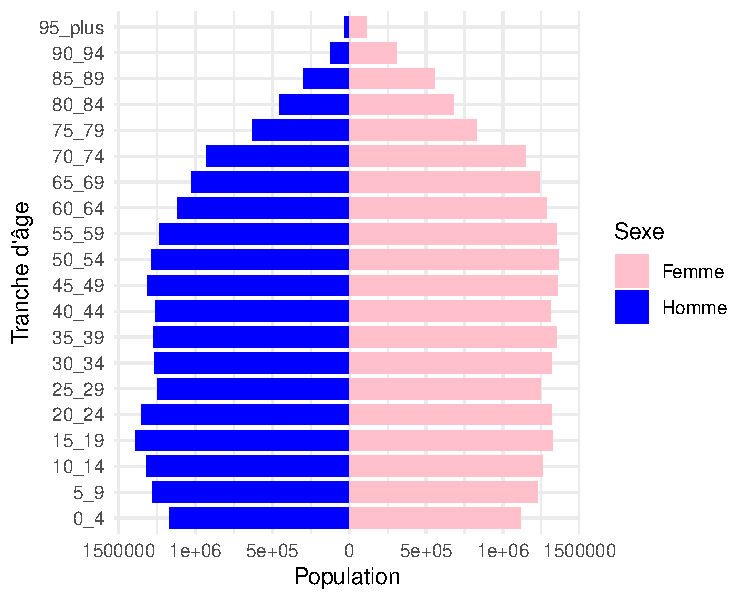
\includegraphics{rapport_intermediaire_files/figure-latex/unnamed-chunk-16-1} 

}

\caption{Pyramide des âges}\label{fig:unnamed-chunk-16}
\end{figure}

Dans cette partie, nous allons réaliser quelques statistiques
descriptives sur nos données.

\subsection{Analyse univariée}\label{analyse-univariuxe9e}

\begin{table}[H]
\centering
\caption{\label{tab:unnamed-chunk-17}Résumé statistique du nombre de visites}
\centering
\begin{tabular}[t]{rrrrrr}
\toprule
Min. & 1st Qu. & Median & Mean & 3rd Qu. & Max.\\
\midrule
\cellcolor{gray!10}{1037} & \cellcolor{gray!10}{5993} & \cellcolor{gray!10}{9127} & \cellcolor{gray!10}{19129.63} & \cellcolor{gray!10}{17290} & \cellcolor{gray!10}{765833}\\
\bottomrule
\end{tabular}
\end{table}

\begin{enumerate}
\def\labelenumi{\arabic{enumi}.}
\tightlist
\item
  Taux et Nombre de visites
\end{enumerate}

L'analyse des statistiques descriptives sur le nombre de consultations
annuelles de médecin généraliste entre 2018 et 2022 révèle une
distribution fortement asymétrique à droite, avec une grande dispersion
des données. La moyenne de 19130 consultations, nettement supérieure à
la médiane de 9127, indique la présence de valeurs extrêmes tirant la
distribution vers le haut. Cette asymétrie est confirmée par l'écart
considérable entre le minimum de 1037 et le maximum de 765833
consultations par an.

La moitié des médecins généralistes effectuent entre 5993 et 17290
consultations annuellement, ce qui suggère une variabilité importante
dans la charge de travail. La médiane de 9127 consultations par an,
équivalant à environ 25 consultations par jour ouvrable, semble plus
représentative de l'activité typique d'un médecin généraliste que la
moyenne influencée par les valeurs extrêmes. Ces statistiques mettent en
lumière la diversité des pratiques et des charges de travail parmi les
médecins généralistes, avec potentiellement quelques cas atypiques
présentant un volume de consultations exceptionnellement élevé.

Le nombre de visites pouvant potentiellement être influencé par la
taille de la commune et donc par sa population, nous avons éliminer cet
effet en calculant le taux de consultations qui n'est autre que le
nombre de consultations moyennes par personnes.

\begin{enumerate}
\def\labelenumi{\arabic{enumi}.}
\setcounter{enumi}{1}
\tightlist
\item
  Taux de mortalité et de Natalité
\end{enumerate}

Dans les commmunes étudiées, le taux de natalité et de mortalité sont un
peu élevées avec la plupart des taux variant entre 5 et 15 pour 1000 en
ce qui concerne la natalité et 0 et 20 pour 1000 pour la mortalité. On
remarque une corrélation négative entre ces deux taux. Néanmoins cette
corrélation n'a à priori aucun sens. Par ailleurs, l'observation des
distribution permet de constater que la natalité est nde façon générale
élevée par rapport à la mortalité dans les communes étudiées.

\begin{figure}

{\centering 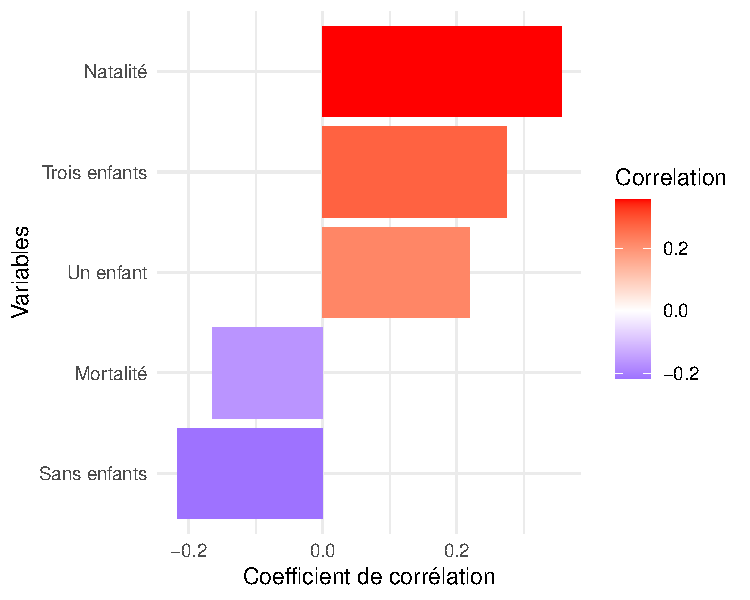
\includegraphics{rapport_intermediaire_files/figure-latex/unnamed-chunk-18-1} 

}

\caption{Taux de Natalité et Taux de Mortalité}\label{fig:unnamed-chunk-18}
\end{figure}

\begin{figure}

{\centering 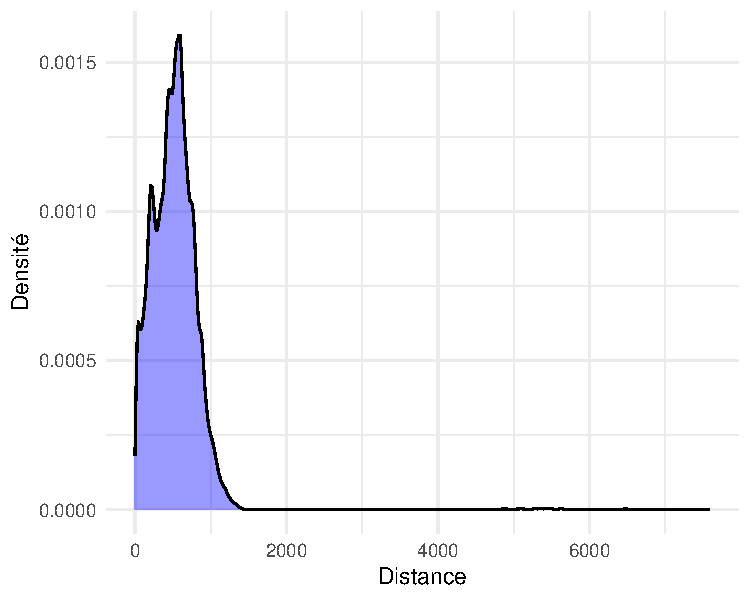
\includegraphics{rapport_intermediaire_files/figure-latex/unnamed-chunk-19-1} 

}

\caption{Répartition du nombre et du taux de consultations}\label{fig:unnamed-chunk-19}
\end{figure}

\subsection{Analyse bivariée}\label{analyse-bivariuxe9e}

Nous allons ici, voir s'il y a un lien à priori entre le taux de
consultation et certaines de nos variables explicatives. Ainsi, nous
avons d'abord réalisé une analyse descriptive bivariée puis nous avons
calculé la corrélation de Pearson pour évaluer le lien linéaire entre le
taux de consulation et des variables telles que la population totale, la
part des personnes agées (75 ans et plus), la part de quelques CSP
(ouvriers et retraités).

\subsubsection{Taux de consultation et population
totale}\label{taux-de-consultation-et-population-totale}

\(\\\)

\begin{table}[H]
\centering
\caption{\label{tab:unnamed-chunk-20}Taux de consultations selon la taille de la commune}
\centering
\begin{tabular}[t]{lr}
\toprule
taille\_commune & Taux de consulations\\
\midrule
\cellcolor{gray!10}{Grande (> 8974)} & \cellcolor{gray!10}{1.526810}\\
Moyenne (4849 - 8974) & 1.456356\\
\cellcolor{gray!10}{Petite (<= 4848)} & \cellcolor{gray!10}{1.383861}\\
\bottomrule
\end{tabular}
\end{table}

En divisant les communes en trois groupes égaux (ou presque égaux) en
fonction de la population totale, il ressort qu'en moyenne, plus la
taille de la commune est importante plus le taux de consulations est
élevé.

\subsubsection{Taux de consultation et population
âgée}\label{taux-de-consultation-et-population-uxe2guxe9e}

\begin{table}[H]
\centering
\caption{\label{tab:unnamed-chunk-21}Taux de consultations selon la population âgée}
\centering
\begin{tabular}[t]{lr}
\toprule
population\_agee\_importante & consultations\_moyennes\\
\midrule
\cellcolor{gray!10}{Non (<= 670)} & \cellcolor{gray!10}{1.501111}\\
Oui (> 670) & 1.410213\\
\bottomrule
\end{tabular}
\end{table}

\begin{figure}

{\centering 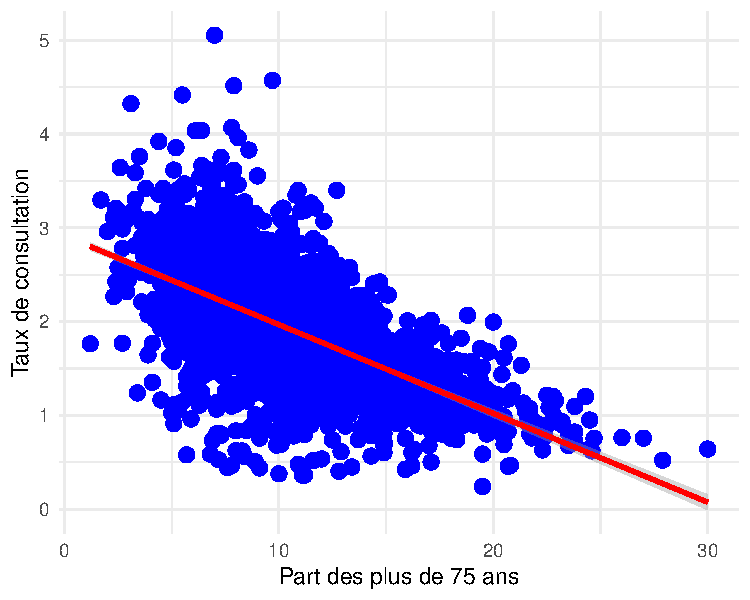
\includegraphics{rapport_intermediaire_files/figure-latex/unnamed-chunk-22-1} 

}

\caption{Relation entre taux de consultations et part des plus de 75 ans}\label{fig:unnamed-chunk-22}
\end{figure}

Les communes avec une population âgée importante (communes dont la
population âgée de 75 ans ou plus est supérieure à la médiane) ont en
moyenne un taux de consultations plus faible.

\subsubsection{Taux de consultation et
CSP}\label{taux-de-consultation-et-csp}

Aucune catégorie ne semble montrer une relation linéaire évidente avec
le taux de visite. Par ailleurs, pour toutes les catégories
socio-professionnelles, la majorité des communes se situent dans une
plage de proportions faibles, ce qui limite la variabilité observable
dans les relations. Une analyse statistique supplémentaire, comme le
calcul de corrélations, serait nécessaire pour confirmer ou infirmer les
relations observées visuellement.

\subsubsection{Analyse de corrélation}\label{analyse-de-corruxe9lation}

Les résultats de la corrélation de Pearson sont consignées dans le
tableau suivant :

\begin{table}[H]
\centering
\caption{\label{tab:unnamed-chunk-24}Corrélations de Pearson entre le taux de consultation et les autres variables}
\centering
\begin{tabular}[t]{llrrl}
\toprule
  & Variable & Correlation & P\_value & Significatif\\
\midrule
\cellcolor{gray!10}{cor} & \cellcolor{gray!10}{population\_municipale\_2021\_x} & \cellcolor{gray!10}{0.0765022} & \cellcolor{gray!10}{0.0000118} & \cellcolor{gray!10}{Oui}\\
cor1 & part\_des\_pers\_agees\_de\_75\_ans\_ou\_2021 & -0.6258560 & 0.0000000 & Oui\\
\cellcolor{gray!10}{cor2} & \cellcolor{gray!10}{population\_de\_15\_ans\_ou\_selon\_la\_csp\_2021\_retraites} & \cellcolor{gray!10}{-0.0285517} & \cellcolor{gray!10}{0.1024362} & \cellcolor{gray!10}{Non}\\
cor3 & population\_de\_15\_ans\_ou\_selon\_la\_csp\_2021\_ouvriers & 0.1077559 & 0.0000000 & Oui\\
\bottomrule
\end{tabular}
\end{table}

Les résultats nous montrent que le taux de consultation est positivement
corrélé à la population ainsi qu'à celle de plus de 15 ans. Cependant la
corrélation est faible. Par ailleurs, la corrélation est négative avec
la part des personnes agées de plus de 75 ans. Cela dit, plus la part
des plus de 75 ans augmente moins est le taux de consultations dans une
commune. Cela peut vouloir dire que les personnes de plus de 75 ans sont
ceux qui ne se consultent pas assez.

\begin{figure}

{\centering 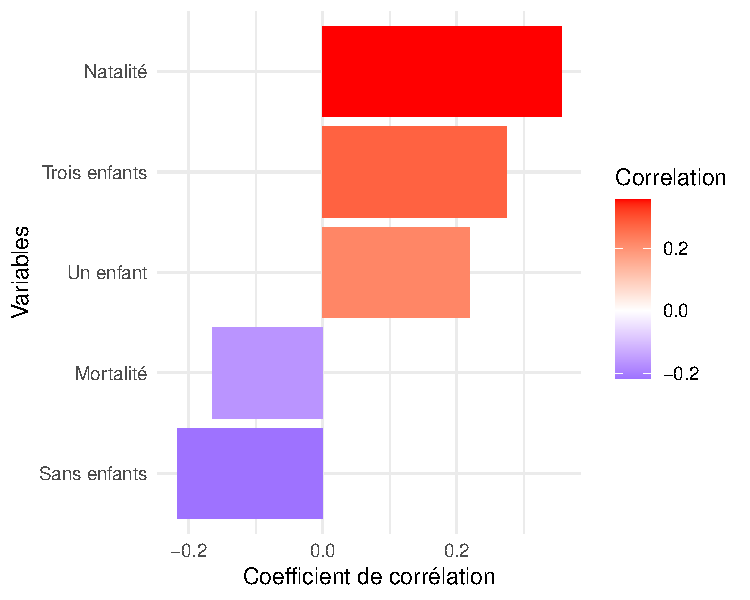
\includegraphics{rapport_intermediaire_files/figure-latex/unnamed-chunk-25-1} 

}

\caption{Corrélations entre le nombre de visite et quelques variables}\label{fig:unnamed-chunk-25}
\end{figure}

\subsection{Autocorrélation}\label{autocorruxe9lation}

L'autocorrélation spatiale est une mesure essentielle pour analyser la
dépendance entre des observations géographiques. Dans notre étude nos
données sont des données portant sur des communes. Ainsi il peut exister
une dépendance entre nos taux de consultations du fait de la proximité
des communes ou de l'appartenance à un même département ou région. Ainsi
nous allons mesurer cette dépendance en évaluant l'autocorrélation
spatiale. Dans ce contexte, \textbf{l'indice de Moran} est largement
utilisé pour quantifier cette dépendance en fournissant une mesure
globale de l'autocorrélation spatiale.

\subsubsection{Définition de l'indice de
Moran}\label{duxe9finition-de-lindice-de-moran}

L'indice de Moran (\(I\)) évalue la similitude des valeurs d'une
variable entre différentes entités géographiques (par exemple, des
communes) en fonction de leur proximité spatiale. Il se base sur la
matrice de poids spatiale (\(W\)), qui définit les relations entre ces
entités.

\subsubsection{Formule de l'indice de
Moran}\label{formule-de-lindice-de-moran}

La formule mathématique de l'indice de Moran est la suivante :

\[
I = \frac{n}{\sum_{i=1}^n \sum_{j=1}^n w_{ij}} \cdot \frac{\sum_{i=1}^n \sum_{j=1}^n w_{ij} (x_i - \bar{x})(x_j - \bar{x})}{\sum_{i=1}^n (x_i - \bar{x})^2}
\]

Où :

\begin{itemize}
\item
  \(n\) : Nombre total d'entités spatiales (Ici, le nombre de communes).
\item
  \(x_i, x_j\) : Valeurs observées de la variable pour les entités \(i\)
  et \(j\) (Ici le taux de consultations)
\item
  \(\bar{x}\) : Moyenne de la variable \(x\).
\item
  \(w_{ij}\) : Poids spatial définissant la relation entre \(i\) et
  \(j\).
\end{itemize}

La matrice de \(W\) peut être constuit sur la base du voisinage entre
les deux communes ou soit de la distance entre les deux communes. Dans
le premier cas alors \(w_{ij}\) \(w_{ij} = 1\) si \(i\) et \(j\) sont
voisins et \(w_{ij} = 0\) sinon. Dans le second cas \(w_{ij} = d_{ij}\).
Nous allons dans notre cas utiliser une matrice de poids basée sur la
distance, notamment celle d'Haversine.

\subsubsection{Matrice de poids basée sur la distance de
Haversine}\label{matrice-de-poids-basuxe9e-sur-la-distance-de-haversine}

La distance de Haversine est une mesure de la distance entre deux points
sur une sphère, basée sur leurs coordonnées géographiques (\(latitude\)
et \(longitude\)). Elle est particulièrement utile pour les données
géographiques projetées sur une surface sphérique, comme la Terre.

\subsubsection{Formule de la distance de
Haversine}\label{formule-de-la-distance-de-haversine}

Si l'on considère deux points (\(i\)) et (\(j\)), la distance
(\(d_{ij}\)) entre ces deux points sur la surface d'une sphère de rayon
(\(r\)) est donnée par :

\[
 d_{ij} = 2r \cdot \arcsin\left(\sqrt{\sin^2\left(\frac{\phi_j - \phi_i}{2}\right) + \cos(\phi_i)\cos(\phi_j)\sin^2\left(\frac{\lambda_j - \lambda_i}{2}\right)}\right)
\]

Où :

\begin{itemize}
\item
  \(r\) : Rayon de la Terre (environ 6371 km).
\item
  \(\phi_i, \phi_j\) : Latitudes des points \(i\) et \(j\) (en radians).
\item
  \(\lambda_i, \lambda_j\) : Longitudes des points \(i\) et \(j\) (en
  radians). Après calcul nous avons ces statistiques sur nos distances.
\end{itemize}

Une visualtion de la densité de nos distance nous donne ceci, indiquant
une forte asymétrie à gauche de la distribution. En d'autres termes,les
communes étudiées sont assez rapprochées les unes des autres pour la
plupart.

\begin{figure}

{\centering 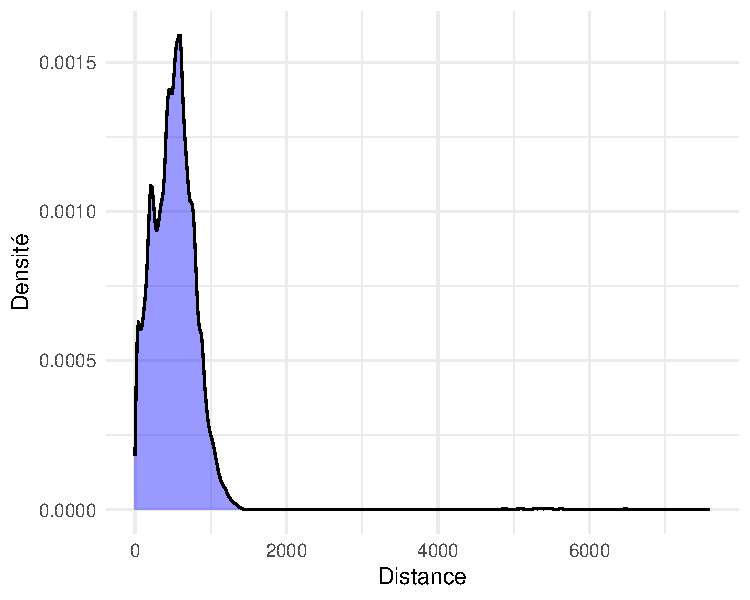
\includegraphics{rapport_intermediaire_files/figure-latex/unnamed-chunk-27-1} 

}

\caption{Densité des distances}\label{fig:unnamed-chunk-27}
\end{figure}

\subsubsection{Construction de la matrice de
poids}\label{construction-de-la-matrice-de-poids}

\hfill\break
Pour construire la matrice de poids, nous avons alors suivi ces
étapes.\\

\begin{enumerate}
\def\labelenumi{\arabic{enumi}.}
\tightlist
\item
  Calculer les distances de Haversine entre chaque paire d'entités.
\item
  Définir un seuil de distance maximale (\(d_{max}\)) :

  \begin{itemize}
  \tightlist
  \item
    Si \(d_{ij} < d_{max}\), \(w_{ij} = \frac{1}{d_{ij}}\).
  \item
    Sinon, \(w_{ij} = 0\).
  \end{itemize}
\item
  Normaliser les poids pour que chaque ligne de la matrice ait une somme
  égale à 1 : \[
   w_{ij}^{norm} = \frac{w_{ij}}{\sum_{j} w_{ij}}.
  \]
\end{enumerate}

\begin{table}[H]
\centering
\caption{\label{tab:unnamed-chunk-28}Résultats du test de Moran}
\centering
\begin{tabular}[t]{lr}
\toprule
  & x\\
\midrule
\cellcolor{gray!10}{Moran I statistic} & \cellcolor{gray!10}{0.1275832}\\
Expectation & -0.0003056\\
\cellcolor{gray!10}{Variance} & \cellcolor{gray!10}{0.0000029}\\
\bottomrule
\end{tabular}
\end{table}

Ainsi dans notre étude, nous avons trouvé un indice de Moran égale à
0.1275832. Le test nous a permi d'obtenir une p-value de 0. Ce qui
permet de conclure qu'il y a effectivement une autocorrélation positive
et significative entre les communes selon leur taux de consultations.

\section{Annexes}\label{annexes}

\begin{figure}
    \centering
    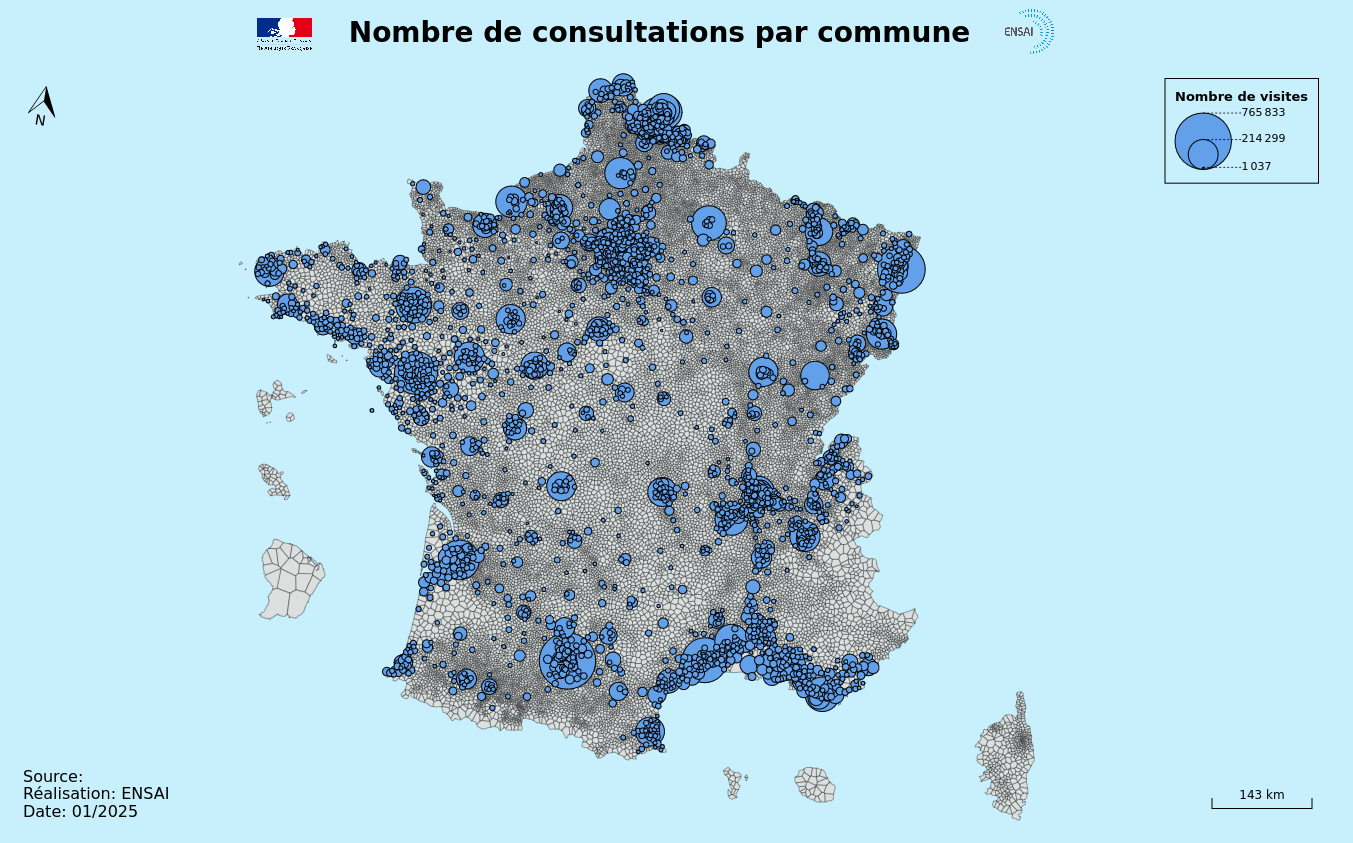
\includegraphics[width=1\linewidth]{../cartes/nombre_de_consulatations}
    \caption{Carte du nombre de consultations par commune}
    \label{fig:figure}
\end{figure}
\begin{figure}
    \centering
    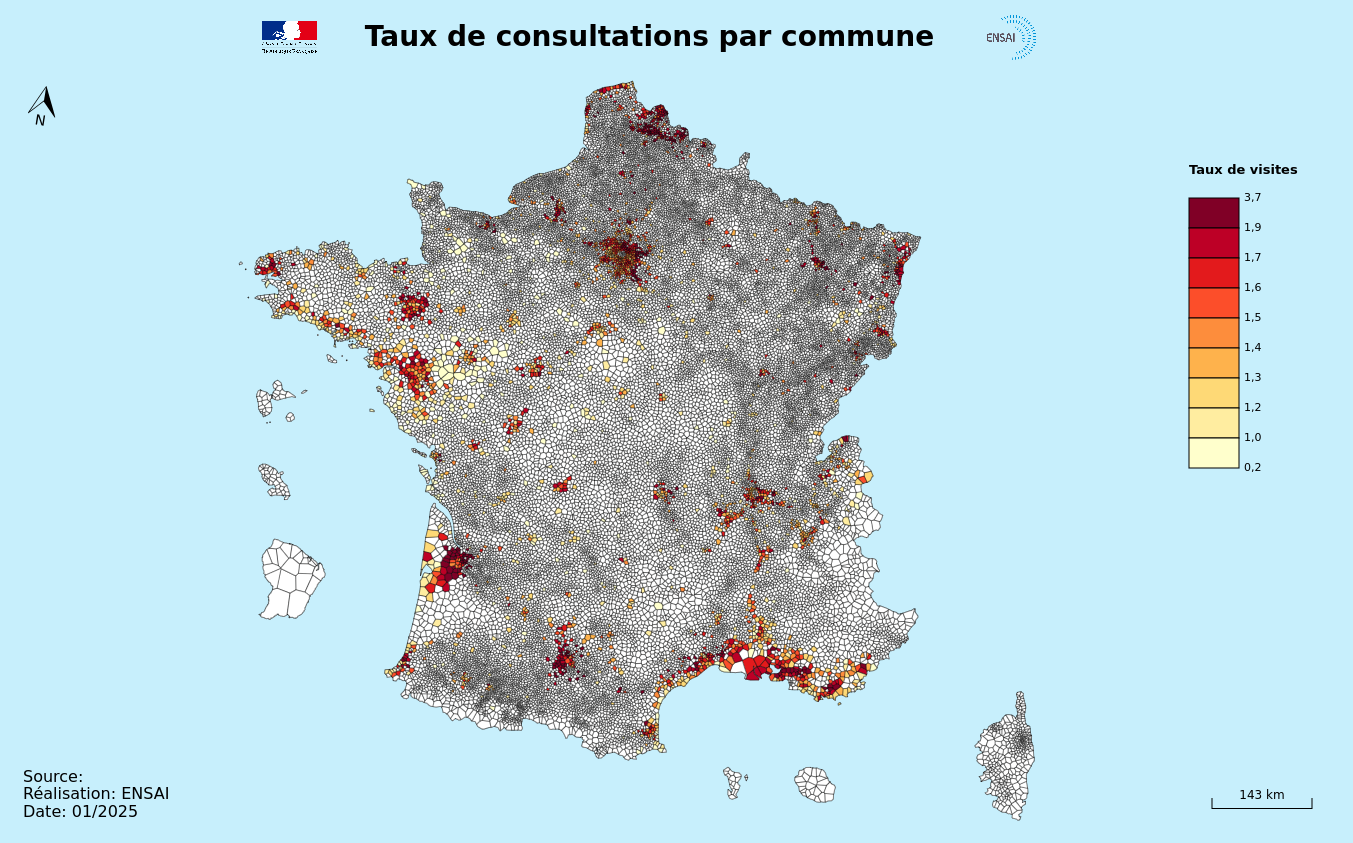
\includegraphics[width=1\linewidth]{../cartes/taux_de_consultations}
    \caption{Carte du taux de consultations par commune}
    \label{fig:figure}
\end{figure}
\begin{figure}
    \centering
    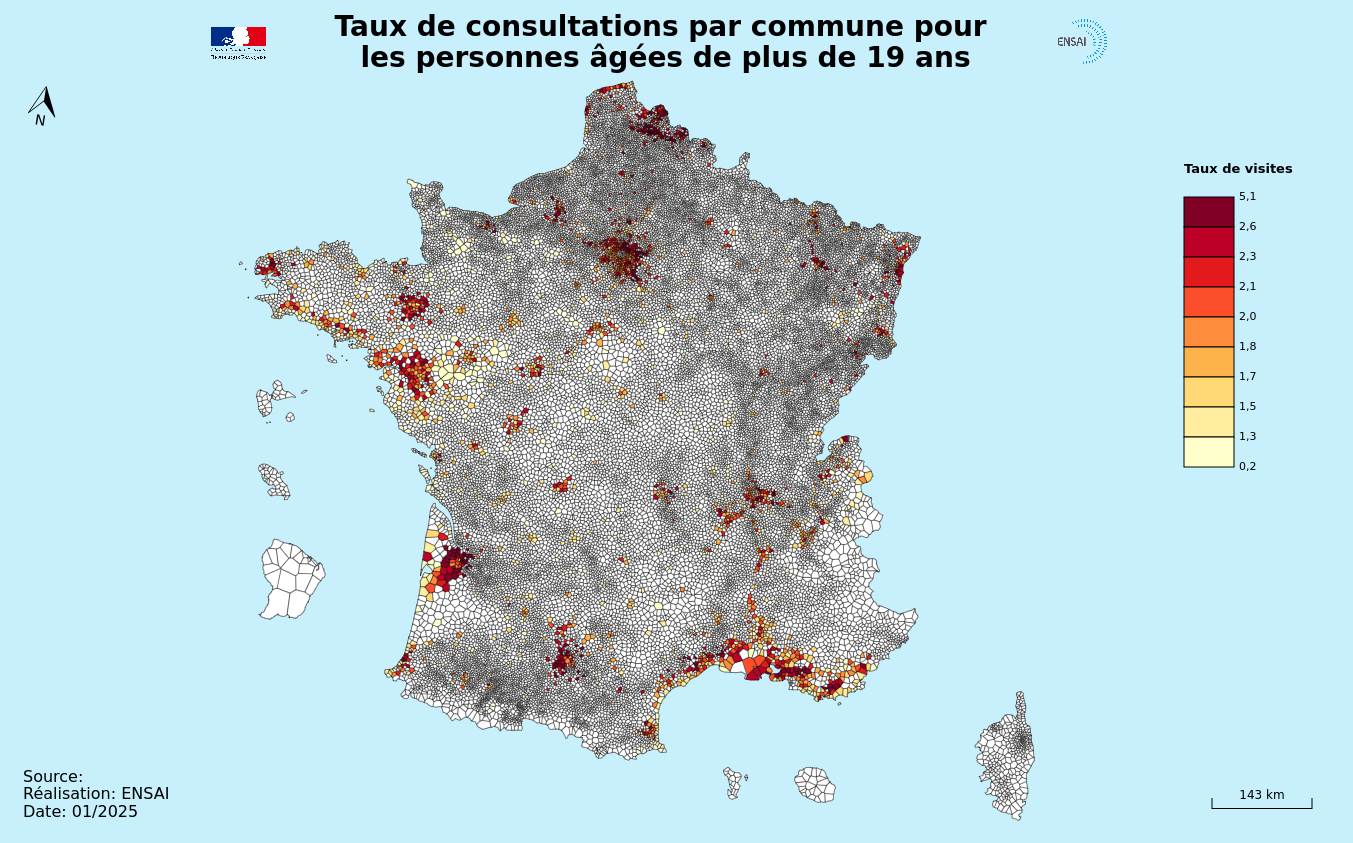
\includegraphics[width=1\linewidth]{../cartes/taux_de_consultations_plus_19_ans}
    \caption{Carte du taux de consultations par commune pour les plus de 19 ans}
    \label{fig:figure}
\end{figure}

\phantomsection\label{refs}
\begin{CSLReferences}{1}{0}
\bibitem[\citeproctext]{ref-statcan2022}
Canada, Statistique. 2022. {«~Fréquence des consultations médicales et
facteurs sociodémographiques~»}. \url{https://www150.statcan.gc.ca}.

\bibitem[\citeproctext]{ref-irdes2020}
Irdes. 2020. {«~Inégalités spatiales d'accessibilité aux soins
médicaux~»}. \url{https://www.irdes.fr}.

\bibitem[\citeproctext]{ref-bag2024}
publique, Office fédéral de la santé. 2024. {«~Santé des femmes et accès
aux soins en Suisse~»}. \url{https://bag.admin.ch}.

\bibitem[\citeproctext]{ref-bvs2023}
Santé, BVS. 2023. {«~Facteurs influençant l'accès aux soins médicaux en
milieu défavorisé~»}. \url{https://docs.bvsalud.org}.

\end{CSLReferences}

\end{document}
